\documentclass [9 pt]{article}
\usepackage[margin = 1in]{geometry}
\usepackage{amsfonts}
\usepackage{amsthm}
\usepackage{bbm}
 \usepackage{amsmath}
\usepackage[utf8]{inputenc}
\usepackage{graphicx}
\usepackage{enumerate}
\usepackage{color}
\usepackage{graphicx}
\graphicspath{ {./images/} }
\usepackage{tikz}

\theoremstyle{definition}
\newtheorem{problem}{Problem}
\newtheorem{theorem}{Theorem}
\newtheorem*{corollary}{Corollary}
\newtheorem{proposition}[theorem]{Proposition}
\newtheorem{lemma}[theorem]{Lemma}
\newtheorem{conjecture}[theorem]{Conjecture}

\newtheorem{definition}[theorem]{Definition}
\newtheorem{remark}[theorem]{Remark}
\newtheorem{example}[theorem]{Example}


\usepackage{fancyhdr}
\pagestyle{fancy}
\lhead{Yuhao Wu \quad 260711365} 
\rhead{\bfseries COMP 330 Assignment 1}
\cfoot{\thepage}
\renewcommand{\headrulewidth}{0.4pt}
\renewcommand{\footrulewidth}{0.4pt}





\begin{document}

\title{COMP 330 Assignment 1}
\date{2018-9-15}
\author{Name: Yuhao Wu\\
ID Number: 260711365
}
\maketitle

\section*{Question 1:}
Fix a finite alphabet $\sum$ and let $\emptyset \neq L \subseteq \sum^{*}$. We define the following relation R on words from $\sum^{*}:$
$$ \forall x, y \in \Sigma^{*}, xRy \text{ if }\forall z \in \Sigma^{*}, xz \in L \text{ iff } yz \in L $$
Prove that this is an equivalence relation.
\begin{proof}
	$$ \forall x, y \in \Sigma^{*}, xRy \text{ if }\forall z \in \Sigma^{*}, xz \in L \text{ iff } yz \in L $$
	%$$ \text{ This can be translated into }\quad \quad \bigg[  \forall x, y \in \Sigma^{*} \text{ and } \forall z \in \Sigma^{*}, xz \in L \Leftrightarrow yz \in L \bigg] \implies xRy $$%
	
	As we need to prove this is an equivalence relation, we need to prove that:
	(1) reflexivity (2) symmetry (3) transitivity\\
	\begin{itemize}
		\item reflexivity: we need to show   $\forall x \in \Sigma^{*}, xRx$\\
		$ \forall  z \in \Sigma^{*}, xz \in L \Leftrightarrow xz \in L $ (I think this is obvious, no more proof), according the relation $R$ defined in the question, we can imply that $xRx$
		\item symmetry: we need to show  $\forall x, y \in \Sigma^{*}, xRy \implies yRx$\\
		\begin{align*}
			\bigg[\forall z \in \Sigma^{*}, xz \in L \Leftrightarrow yz \in L\bigg] &\implies \bigg[\forall z \in \Sigma^{*}, yz \in L \Leftrightarrow xz \in L\bigg]\\
			xRy &\implies yRx
		\end{align*}
		\item transitivity: we need to show $\forall x, y, z\in \Sigma^{*}, xRy, yRz \implies xRz$\\
		This is equivalent to if we have:
			$$(1)\bigg[\forall w \in \Sigma^{*}, xw \in L \Leftrightarrow yw \in L\bigg] \quad \quad (2) \bigg[\forall w \in \Sigma^{*}, yw \in L \Leftrightarrow zw \in L\bigg] $$
			$$\text{could we imply that: } \bigg[\forall w \in \Sigma^{*}, xw \in L \Leftrightarrow zw \in L\bigg] $$
			Suppose $w$ is some word in $\Sigma^{*}$ and suppose that $xw \in L$, then (1) tells us that $yw \in L$. If $yw \in L$,  (2) tells us that $zw \in L$. Thus $xw \in L \implies zw \in L$.\\
			Suppose $w$ is some word in $\Sigma^{*}$ and suppose that $zw \in L$, then (2) tells us that $yw \in L$. If $yw \in L$,  (1) tells us that $xw \in L$. Thus $zw \in L \implies xw \in L$.\\
			Thus, we can say that: 
			\begin{align*}
					(1)\bigg[\forall w \in \Sigma^{*}, xw \in L \Leftrightarrow yw \in L\bigg] \quad \quad (2) \bigg[\forall w \in \Sigma^{*}, yw \in L \Leftrightarrow zw \in L\bigg] 
					&\implies \bigg[\forall w \in \Sigma^{*}, xw \in L \Leftrightarrow zw \in L\bigg]\\
					\forall x, y, z\in \Sigma^{*}, xRy, yRz &\implies xRz
			\end{align*}   
	\end{itemize} 
\end{proof}
\newpage
\section*{Question 2: }
Consider, pairs of natural numbers $< m,n >$ where $m, n \in \mathbb{N}$. We order them by the relation \\
$<m, n> \sqsubseteq <m',n'> \text{ if } m < m' \text{ or }(m = m') \wedge (n \leq n')$, where $\leq$ is the usual numerical order.\\
(1): Prove that the relation $\sqsubseteq$ is a partial order.\\
(2): Prove that the relation $\sqsubseteq$ is a well-founded order.\\
\newline
\textbf{(1):}\\
\begin{proof}
	We need to  prove (1) reflexive, (2) antisymmetric, (3) transitive.
	\begin{itemize}
		\item To begin with, we need to prove that $ \forall s = <m, n>, s\sqsubseteq  s $\\
		Obviously, we have $(m = m) \wedge (n \leq n)$ which implies that $s \sqsubseteq s $
		\item Then, we need to prove that $ \forall s = <m ,n>\text{ and } t = <m', n'>, s \sqsubseteq t \text{ and } t \sqsubseteq s \implies s = t  $\\
		If $s \sqsubseteq t $, then we say that $  m < m' \text{ or }(m = m') \wedge (n \leq n') $\\
		If $t \sqsubseteq s $, then we say that $  m' < m \text{ or }(m' = m) \wedge (n' \leq n) $\\
		For  $s \sqsubseteq t $, if we choose $m < m'$, we will find it is impossible to conclude $t \sqsubseteq s$. It is the same for $t \sqsubseteq s$.
		\begin{align*}
		&\quad \quad \quad	s \sqsubseteq t \text{ and } t \sqsubseteq s \\
		&\implies \bigg[(m = m') \wedge (n \leq n')\bigg] \wedge \bigg[ (m' = m) \wedge (n' \leq n) \bigg]\\
		&\implies  (m = m') \wedge (n \leq n') \wedge (n' \leq n)\\
		&\implies  (m = m') \wedge (n = n')\\
		&\implies  s = t
		\end{align*} 
		\item In the last, we need to prove that $$ \forall s = <m ,n>, t = <m', n'>,\text{ and } r = <m'', n''> s \sqsubseteq t \text{ and } t \sqsubseteq r \implies s \sqsubseteq r  $$ 
				If $s \sqsubseteq t $, then we say that $  m < m' \text{ or }(m = m') \wedge (n \leq n') $\\
		If $t \sqsubseteq r $, then we say that $  m' < m'' \text{ or }(m' = m'') \wedge (n' \leq n'') $\\
		\newline
		For $s \sqsubseteq t$, if $m < m'$: as for $t \sqsubseteq r, m' \leq m'' $ must hold, we can conclude that $ m < m'' $ , which tells us that $s \sqsubseteq t$\\
		\newline
		For $s \sqsubseteq t$, if $ (m = m') \wedge (n \leq n') $: as for $t \sqsubseteq r: \quad$ \\
		(1)if $m' < m'' $, then we can conclude that: $m < m'' $, which tells us $s \sqsubseteq r $\\
		(2)if $ (m' = m'') \wedge (n' \leq n'') $, then we can conclude that: $ (m = m'') \wedge (n \leq n'') $, which tells us $s \sqsubseteq r$\\
		\newline
		So, we can conclude that: 
		 $$ \forall s = <m ,n>, t = <m', n'>,\text{ and } r = <m'', n''> s \sqsubseteq t \text{ and } t \sqsubseteq r \implies s \sqsubseteq r  $$    
	\end{itemize}
	Thus, we can say that the relation $\sqsubseteq$ is a partial order. 
\end{proof}
\textbf{(2):}\\
\begin{proof}
	Suppose that all the pairs of natural numbers $<m, n>$ where $m, n \in \mathbb{N}$ make up the set $W$.\\
	\newline
	We want to prove that the relation $\sqsubseteq$ is a well-founded order, which is to prove that:
	$$\text{For every non-empty subset } U \text{ of } W, (U \neq \emptyset \quad \&\&\quad U \subseteq W), \exists u_0 \in U \text{ such that } u_0 \text{ is minimal in }U.$$\\
	Suppose that there are $k$ elements in the set $U$. As  $(\mathbb{N}, \leq)$ is well-founded, we can always find the minimal $m_0$ among the k pairs.\\
	\newline
	It is possible that there are j pairs of $<m, n>$, where $m_1 = m_2 = \ldots = m_j = \text{minimal among the k elements}$\\
	\newline
	As  $(\mathbb{N}, \leq)$ is well-founded, we can always find the minimal $n_0$ among the j pairs.\\
	\newline
	In this case, we can say that $u_0 = <m_0, n_0>$ is the minimal among all the k elements in the set $U$.\\
	\newline
	Suppose $u_i = <m_i, n_i>$ is any element among the k elements. \\Due to the way we construct $u_0$, $m_0 \leq m_i$.
	If $m_0 < m_i$, according to the definition, we can say $u_0 \sqsubseteq u_i$\\
	If $ m_o = m_i$, due to the way we construct $u_0$, $n_0 \leq n_i$, according to the definition $( m_0 = m_i) \wedge (n_0 \leq n_i)$ , we can say $ u_0 \sqsubseteq u_i $\\
	\newline
	Thus, we can say that there is nothing smaller than $u_0$, so $u_0$ is minimal in set $U$.

	
\end{proof}

\section*{Question 3:}
\subsection*{(1):}
\begin{center}
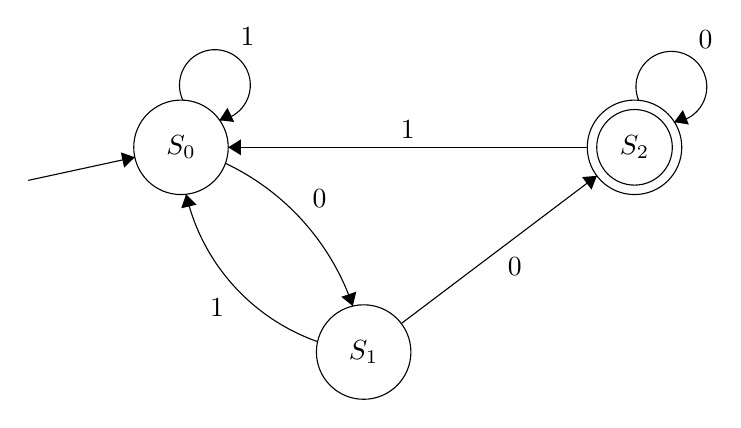
\begin{tikzpicture}[scale=0.2]
\tikzstyle{every node}+=[inner sep=0pt]
\draw [black] (15,-23.1) circle (3);
\draw (15,-23.1) node {$S_0$};
\draw [black] (26.6,-36.1) circle (3);
\draw (26.6,-36.1) node {$S_1$};
\draw [black] (43.8,-23.1) circle (3);
\draw (43.8,-23.1) node {$S_2$};
\draw [black] (43.8,-23.1) circle (2.4);
\draw [black] (5.3,-25.2) -- (12.07,-23.73);
\fill [black] (12.07,-23.73) -- (11.18,-23.42) -- (11.39,-24.39);
\draw [black] (15.122,-20.114) arc (205.38954:-82.61046:2.25);
\draw (19.23,-16.67) node [above] {$1$};
\fill [black] (17.44,-21.38) -- (18.38,-21.49) -- (17.95,-20.59);
\draw [black] (17.819,-24.114) arc (64.70136:18.78419:15.583);
\fill [black] (25.91,-33.18) -- (26.13,-32.27) -- (25.18,-32.59);
\draw (23.33,-26.37) node [right] {$0$};
\draw [black] (28.99,-34.29) -- (41.41,-24.91);
\fill [black] (41.41,-24.91) -- (40.47,-24.99) -- (41.07,-25.79);
\draw (36.2,-30.1) node [below] {$0$};
\draw [black] (44.065,-20.123) arc (202.64196:-85.35804:2.25);
\draw (48.31,-16.84) node [above] {$0$};
\fill [black] (46.32,-21.5) -- (47.25,-21.65) -- (46.87,-20.73);
\draw [black] (40.8,-23.1) -- (18,-23.1);
\fill [black] (18,-23.1) -- (18.8,-23.6) -- (18.8,-22.6);
\draw (29.4,-22.6) node [above] {$1$};
\draw [black] (23.68,-35.44) arc (-109.3647:-167.14974:12.987);
\fill [black] (15.32,-26.08) -- (15.02,-26.97) -- (15.99,-26.74);
\draw (17.76,-33.29) node [left] {$1$};
\end{tikzpicture}
\end{center}
\subsection*{(2):}
\begin{center}
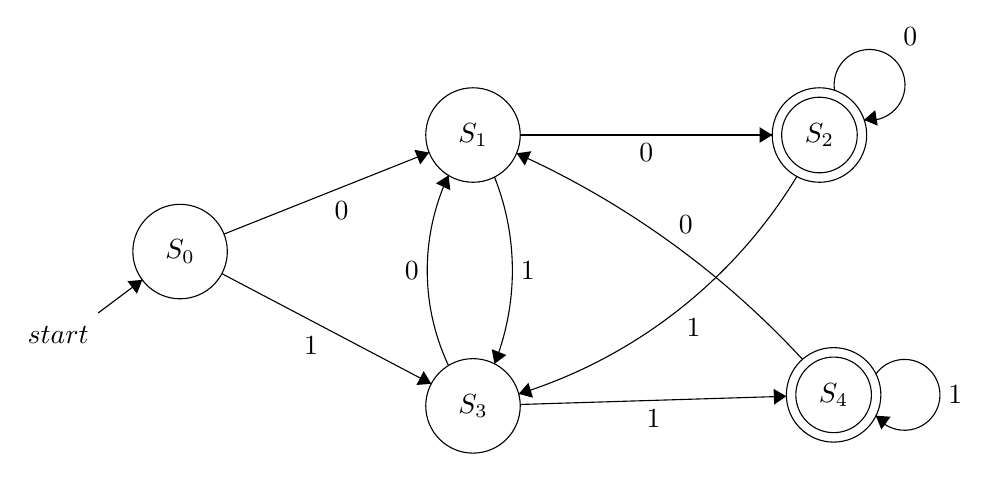
\begin{tikzpicture}[scale=0.2]
\tikzstyle{every node}+=[inner sep=0pt]
\draw [black] (10.9,-22.9) circle (3);
\draw (10.9,-22.9) node {$S_0$};
\draw [black] (29.5,-15.5) circle (3);
\draw (29.5,-15.5) node {$S_1$};
\draw [black] (51.5,-15.5) circle (3);
\draw (51.5,-15.5) node {$S_2$};
\draw [black] (51.5,-15.5) circle (2.4);
\draw [black] (29.5,-32.7) circle (3);
\draw (29.5,-32.7) node {$S_3$};
\draw [black] (52.4,-32) circle (3);
\draw (52.4,-32) node {$S_4$};
\draw [black] (52.4,-32) circle (2.4);
\draw [black] (5.7,-26.8) -- (8.5,-24.7);
\draw (5.12,-28.2) node [left] {$start$};
\fill [black] (8.5,-24.7) -- (7.56,-24.78) -- (8.16,-25.58);
\draw [black] (13.69,-21.79) -- (26.71,-16.61);
\fill [black] (26.71,-16.61) -- (25.78,-16.44) -- (26.15,-17.37);
\draw (21.15,-19.72) node [below] {$0$};
\draw [black] (32.5,-15.5) -- (48.5,-15.5);
\fill [black] (48.5,-15.5) -- (47.7,-15) -- (47.7,-16);
\draw (40.5,-16) node [below] {$0$};
\draw [black] (52.46,-12.67) arc (189:-99:2.25);
\draw (56.8,-9.25) node [right] {$0$};
\fill [black] (54.33,-14.54) -- (55.2,-14.91) -- (55.04,-13.92);
\draw [black] (55.08,-30.677) arc (144:-144:2.25);
\draw (59.65,-32) node [right] {$1$};
\fill [black] (55.08,-33.32) -- (55.43,-34.2) -- (56.02,-33.39);
\draw [black] (32.5,-32.61) -- (49.4,-32.09);
\fill [black] (49.4,-32.09) -- (48.59,-31.62) -- (48.62,-32.62);
\draw (40.97,-32.88) node [below] {$1$};
\draw [black] (13.55,-24.3) -- (26.85,-31.3);
\fill [black] (26.85,-31.3) -- (26.37,-30.49) -- (25.91,-31.37);
\draw (19.21,-28.3) node [below] {$1$};
\draw [black] (27.945,-30.141) arc (-154.78533:-205.21467:14.18);
\fill [black] (27.95,-18.06) -- (27.15,-18.57) -- (28.06,-19);
\draw (26.09,-24.1) node [left] {$0$};
\draw [black] (30.863,-18.167) arc (21.71403:-21.71403:16.035);
\fill [black] (30.86,-30.03) -- (31.62,-29.47) -- (30.69,-29.1);
\draw (32.5,-24.1) node [right] {$1$};
\draw [black] (50.066,-18.134) arc (-31.28508:-72.67704:31.722);
\fill [black] (32.4,-31.94) -- (33.31,-32.18) -- (33.02,-31.23);
\draw (43.5,-27.15) node [below] {$1$};
\draw [black] (32.266,-16.66) arc (65.7287:42.72399:56.117);
\fill [black] (32.27,-16.66) -- (32.79,-17.44) -- (33.2,-16.53);
\draw (43.01,-21.79) node [above] {$0$};
\end{tikzpicture}
\end{center}

\subsection*{(3):}
\begin{center}
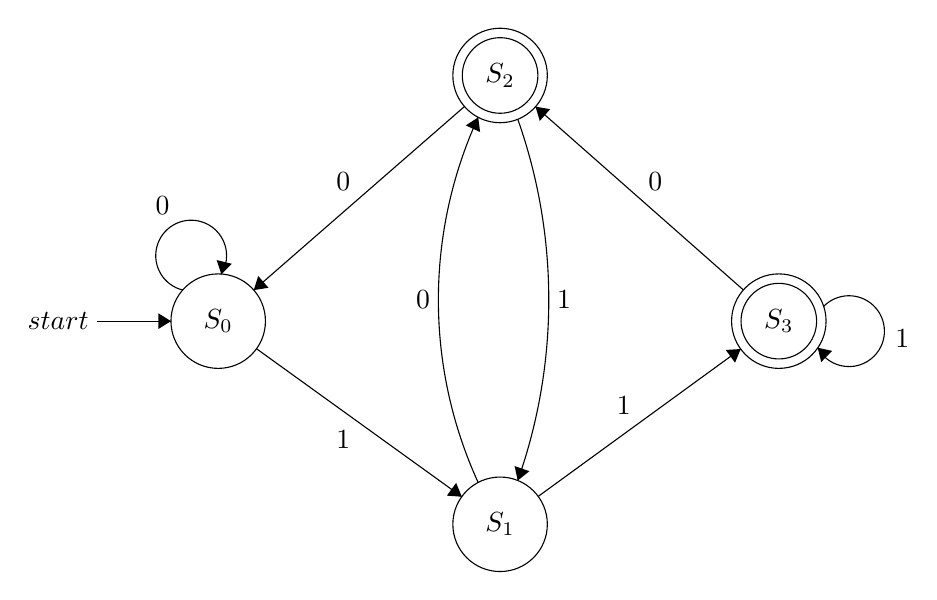
\begin{tikzpicture}[scale=0.2]
\tikzstyle{every node}+=[inner sep=0pt]
\draw [black] (17.2,-30.2) circle (3);
\draw (17.2,-30.2) node {$S_0$};
\draw [black] (35.1,-43.1) circle (3);
\draw (35.1,-43.1) node {$S_1$};
\draw [black] (35.1,-14.6) circle (3);
\draw (35.1,-14.6) node {$S_2$};
\draw [black] (35.1,-14.6) circle (2.4);
\draw [black] (52.8,-30.2) circle (3);
\draw (52.8,-30.2) node {$S_3$};
\draw [black] (52.8,-30.2) circle (2.4);
\draw [black] (14.955,-28.227) arc (256.41851:-31.58149:2.25);
\draw (13.66,-23.44) node [above] {$0$};
\fill [black] (17.4,-27.22) -- (18.07,-26.56) -- (17.1,-26.32);
\draw [black] (9.5,-30.2) -- (14.2,-30.2);
\draw (9,-30.2) node [left] {$start$};
\fill [black] (14.2,-30.2) -- (13.4,-29.7) -- (13.4,-30.7);
\draw [black] (19.63,-31.95) -- (32.67,-41.35);
\fill [black] (32.67,-41.35) -- (32.31,-40.47) -- (31.72,-41.28);
\draw (25.15,-37.15) node [below] {$1$};
\draw [black] (33.707,-40.445) arc (-155.40892:-204.59108:27.862);
\fill [black] (33.71,-17.26) -- (32.92,-17.77) -- (33.83,-18.19);
\draw (30.68,-28.85) node [left] {$0$};
\draw [black] (32.84,-16.57) -- (19.46,-28.23);
\fill [black] (19.46,-28.23) -- (20.39,-28.08) -- (19.74,-27.33);
\draw (25.14,-21.91) node [above] {$0$};
\draw [black] (36.223,-17.381) arc (19.48855:-19.48855:34.378);
\fill [black] (36.22,-40.32) -- (36.96,-39.73) -- (36.02,-39.4);
\draw (38.69,-28.85) node [right] {$1$};
\draw [black] (55.64,-29.27) arc (135.8699:-152.1301:2.25);
\draw (60.17,-31.33) node [right] {$1$};
\fill [black] (55.27,-31.89) -- (55.49,-32.8) -- (56.19,-32.09);
\draw [black] (37.52,-41.33) -- (50.38,-31.97);
\fill [black] (50.38,-31.97) -- (49.43,-32.03) -- (50.02,-32.84);
\draw (42.95,-36.15) node [above] {$1$};
\draw [black] (50.55,-28.22) -- (37.35,-16.58);
\fill [black] (37.35,-16.58) -- (37.62,-17.49) -- (38.28,-16.74);
\draw (44.96,-21.91) node [above] {$0$};
\end{tikzpicture}
\end{center}

\section*{Question 4:}
Suppose that we have a language $L$ described by a DFA $D = \{S, \Sigma, \delta, s_0, F \}$.\\
We can construct a NFA $N = \{ S', \Sigma, \delta', s_0', F' \}$ which recognize LeftHalf:
\begin{itemize}
	\item $S' = S \times S \quad \quad \text{( Cartesian Product)}$
	\item $s_0' = (s_0, f ) \quad \quad (f \in F)$
	\item $F' = \{(s, s)| s \in S  \}$
	\item $\delta' ((s, t), a) = (\delta (s, a), t') \quad \text{where state $t'$ can move to $t$ with at least one single letter in the alphabet  } $
\end{itemize}
EXPLAINATION:
\begin{itemize}
	\item The new state of the NFA is a Cartesian Product of the states of DFA, the first coordinate is for $w_1$ in question and the second is for $w_2$
	\item The start state for the first coordinate is $s_0$, which is the start state of DFA, The start state for the first coordinate is $f \quad f \in F$. We want them to go from two directions and ends in the same state. As they both move the same number of steps, $|w_1| = |w_2|$, and as they end in the same state, which means $w_1 w_2 \in L$
	\item $\delta' ((s, t), a) = (\delta (s, a), t') \quad a \in \Sigma \quad \text{where state $t'$ can move to $t$ with at least one letter in the alphabet  } $
	When we read a letter a from $w_1$, we move $s \text{ to } \delta(s, a)$ and we move $t$ back to $t'$. NOTE: we don't need to know which letter or which path we need to choose, we just need to determine if there is a path so that both $s$ and $t$ can go to the same state. As in the definition, we just need to make sure there \textbf{ exists } $w_2$. 
\end{itemize}
Since a NFA can recognize a regular language, thus, we can say that LeftHalf(L) is regular.

\newpage
\section*{Question 5:}
(1): Give a deterministic finite automaton accepting the following language over the alphabet $\{0, 1\}$: The set of all words containing 100 or 110. \\
\newline
(2): Show that any $DFA$ for recognizing this language must have at least 5 states. 
\subsection*{(1):}
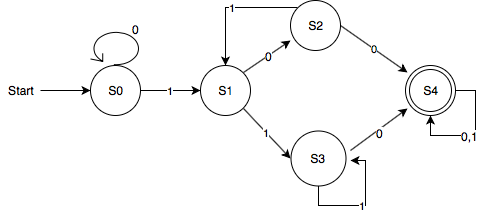
\includegraphics[scale = 0.8]{Q5.png}
\begin{itemize}
	\item $S_0$ means the last three bits are 000
	\item $S_1$ means the last three bits are 001, 101
	\item $S_2$ means the last three bits are 010, when the next is 1, as the automata can't recognize something like 101, so have to go back to $S_1$
	\item $S_3$ means the last three bits are 011, 111, when the next is 1, have to go back to itself
	\item $S_4$ means the word contains 100 or 110, since the automata just wants to recognize words containing 100 or 110, when reading more letters, it stays in $S_4$, which is our accept state.
\end{itemize}
\subsection*{(2):}
\begin{proof}
	As I have already draw a DFA for Question1 using 5 states, what we need to do is to prove that it is impossible for any DFA recognizing this language having only 4 states.\\
	\newline
	As the purpose of the automata is to recognize words containing 100 or 110, which means the automata at least needs to store 3 bits, otherwise how could it be able to recognize 3 bits words.\\
	\newline
	All the possible permutation of 3 bits words is below:
	$$\{000, 001, 010, 011, 100, 101, 110, 111 \}$$
	Obviously, we can separate $\{ 100 , 110 \}$ from above, as they are accept states and others are reject states.\\
	\newline
	Then, we can separate $\{ 010, 011, 111 \}$ from above, as they ends in 11 or 10, when the next bit is 0, they can change into accept states.\\
	But, in fact, we have to separate the three elements, as when the following bits is 1, 010 will change into 101, which is not in this sets.\\
	\newline
	Under this case, we have already had four states:
	\begin{itemize}
		\item $\{100, 110\} \implies$ accepting states
		\item $\{011, 111 \} \implies$ after adding 1, it will still be in this state, after adding 0, it will go to accepting states
		\item  $\{010 \} \implies$ after adding 1, it will go to the fourth state, after adding 0, it will go to accepting states
		\item  $\{ 000, 001, 101 \} $ this is the remaining 
	\end{itemize} 
	For the fourth state, when the next coming bit is 0, 000 will stay in the same states, while 001 and 101 will go to the third state,  and get a contradiction. \\
	So, we can conclude that any $DFA$ for recognizing this language must have at least 5 states. \\
\end{proof}



\end{document}